\documentclass{nitroma-article}
\usepackage[british]{babel}

% page layout
\usepackage{pdflscape}  % landscape pages
\usepackage{afterpage}  % full-page figures at the next opportunity
\usepackage{pdfpages}   % include other PDF docs

% typography
\usepackage{csquotes}   % clever quote marks
    \MakeOuterQuote{"}
\usepackage[detect-all]{siunitx} % numbers and units
    \DeclareSIUnit\year{yr}
    \sisetup{text-celsius = °C}
\usepackage{enumitem}   % control list spacing
    \setlist{noitemsep}
% \usepackage{epigraph}

% formulae
\usepackage{amsmath}
\usepackage{chemmacros} % Swiss-army knife for chemistry

% graphics
\usepackage{graphicx}
\usepackage[font={small,singlespacing},labelfont={bf}]{caption}
\usepackage{subcaption}
\usepackage{wrapfig}
\usepackage{float}
\usepackage{svg}

% tables
\usepackage{tabularx}
\usepackage{booktabs}
\usepackage{multirow}
\usepackage{multicol}
\usepackage{longtable}
\usepackage{colortbl}
\newcommand{\tabsup}[1]{\textsuperscript{\textit{#1}}}

% referencing
\usepackage[hidelinks]{hyperref} % clickable links
    \newcommand{\email}[1]{\href{mailto:#1}{\texttt{#1}}}
\usepackage{cleveref}   % clever cross-referencing
\usepackage[title,titletoc]{appendix}
\usepackage[style=ieee]{biblatex} % references

\title{Interim Design Report: Continuous Nitration of Substituted Aromatics}
\author{Team 8: Marie~Jones, Mathusan~Kandiah, Zong~Lee, Yuxin~Liu, Mustafa~Nasar, Helen~Ogbobi, Wei~Ooi, Andreas~Richardson, Stephen~Tan, Sathurthini~Thurairatnam, Mingchuan~Zheng}
\date{8 February 2021}

\begin{document}

\maketitle

%% !TeX root = ../main.tex
\section*{Executive Summary}
\label{sec:exec-summary}

Substituted aromatic amines are essential intermediates involved in the synthesis of many pharmaceutical compounds, agrochemicals, and dyes \cite{vogt_amines_2000}. The amino group, which cannot be directly introduced via electrophilic aromatic substitution, is instead added via nitration and subsequent reduction. Following multiple deadly industrial accidents in chemical plants performing batch nitration, Chinese authorities are actively attempting to strengthen the control and management of nitration manufacturing \cite{el_diario_china_2019}.

In this context, Nitroma seizes the opportunity; developing an inherently safe, multi-purpose, continuous liquid-phase nitration process to produce o-toluidine, 4-aminobenzaldehyde and 4-aminobenzoic acid. This report details the preliminary design for Nitroma’s demonstration plant, to be located in the Nanjing Chemical Industry Park (China). Synthesis pathways for nitration, oxidation and hydrogenation reactions were selected and modelled in innovative packed-bed microreactors or trickle-bed reactors. Novel downstream processing units, including continuous falling-film melt crystallisers, enable Nitroma to reach the target product purity. Finally, a techno-economic feasibility study was conducted, taking into account health, safety and environmental considerations.

% !TeX root = ../main.tex
\section{Introduction}
\label{sec:introduction}

% !TeX root = ../main.tex
\section{Process Synthesis }
\label{sec:synthesis}
\subsection{Decision analysis}
%explain TOPSIS and AHP
\noindent To make systematic and informed decisions for key aspects of the project, multi-criteria decision making (MCDM) methods were employed. Firstly, pairwise comparison of the criteria was performed with the Analytical Hierarchy Process (AHP) to produce criteria weightings which were fed into the Technique for Order of Preference by Similarity to Ideal Solution (TOPSIS) analysis. Processing of all relevant information through AHP and TOPSIS analysis yielded quantitative rankings for process alternatives, which were initially short-listed with qualitative arguments. Greater importance was given to safety and environmental concerns, technical performance and economic potential.


\subsection{Product selection}
\noindent To deliver a multi-purpose plant, Nitroma selected toluene as feedstock due to the industrial importance of its nitration products and their amino derivatives. All three isomeric nitrotoluenes can indeed easily be oxidised and reduced to substituted aromatic amides of significant importance for the pharmaceutical, agrochemical and textile industries \cite{dugal_nitrobenzene_2005}. Six chemicals were initially selected due to their applications in drugs, fertilizers or dyes \cite{bowers_toluidines_2000,bruhne_benzaldehyde_2011,maki_benzoic_2000}. To determine the three most advantageous products to produce, AHP/TOPSIS analysis was conducted, giving significant importance to the safety of the compounds and their economic potential. Safety was assessed using the NFPA Hazard Classification for health, flammability and instability, where the smallest value is preferable. The economic potential of each chemical was determined using the average price, the average market share of producers which is an indicator of the market share Nitroma can plan to capture, the golbal demand and the expected market growth (CAGR). \Cref{tab:product} summarises the results and the complete methodology can be found in \Cref{app:matrix}.   

\begin{comment}
\noindent To deliver a multi-purpose plant, Nitroma selected toluene as feedstock due to the industrial importance of its nitration products and their amino derivatives. All three isomeric nitrotoluenes can indeed easily be oxidised and reduced to substituted aromatic amides of significant importance for the pharmaceutical, agrochemical and textile industries \cite{dugal_nitrobenzene_2005}. Six chemicals were initially selected due to their applications in drugs, fertilizers or dyes: 2-aminobenzaldehyde (precursor of quinoline derivatives for polymer, agrochemical, dye, antiviral and anti-malaria drug manufacturing), 4-aminobenzaldehyde (intermediate to pharmaceuticals and vanilin), 4-aminobenzoic acid (production of folic acid/vitamin B9), \ortho-toluidine (intermediate in the manufacture of herbicides), \meta-toluidine (manufacture of  photographic color developer) and \para-toluidine (for dye production) \cite{bowers_toluidines_2000,bruhne_benzaldehyde_2011,maki_benzoic_2000}. To determine the three most advantageous products to produce, AHP/TOPSIS analysis was conducted, giving significant importance to the safety of the compounds and their economic potential. Safety was assessed using the NFPA Hazard Classification for health, flammability and instability, where the smallest value is preferable. The economic potential of each chemical was determined using the average price, the average market share of producers which is an indicator of the market share Nitroma can plan to capture, the golbal demand and the expected market growth (CAGR). \Cref{tab:product} summarises the results and the complete methodology can be found in \Cref{app:matrix}.   
\end{comment}


\begin{table}[h]
\centering
    \caption{AHP/TOPSIS results for product selection}
    \label{tab:product}\footnotesize
\begin{tabularx}{\linewidth}{l|S[table-format=4.2]S[table-format=1.1]XS[table-format=7.0,round-mode=figures,round-precision=2]|XX|lll|S[table-format=1.3]S[table-format=1.3]c}
\toprule
                                          & \multicolumn{4}{c}{Economic potential   (29\%)}                                & \multicolumn{2}{|>{\hsize=\dimexpr2\hsize+2\tabcolsep}X}{Process   complexity (14\%)} & \multicolumn{3}{|c|}{EHS (57\%)}     &                       &                          &                           \\ \cmidrule{2-10}
                                          & {\splitcell{Price\\(\si{\USD\per\kg})}} & {\splitcell{CAGR\\(\%)}} & \rcell{Average market share of producer (\%)} & {\splitcell{Demand\\(\si{\tonne\per\year})}} & \rcell{Number of reactions} & \rcell{Max selectivity to toluene (\%)} & \rotatebox[origin=r]{90}{Health} & \rotatebox[origin=r]{90}{Flammability} & \rotatebox[origin=r]{90}{Instability} & AHP & TOPSIS & Rank \\ \midrule
2-aminobenzaldehyde & 1711          & 5.6 & 0.77                           & 1344                 & 2                & 53                       & 2      & 1            & 1           & 0.124                 & 0.273                    & 6                         \\ 
4-aminobenzaldehyde & 19            & 7.1 & 1.75                           & 336842               & 2                 & 44                       & 2      & 1            & 0           & 0.188                 & 0.563                    & \cellcolor{green}2 \\ 
o-toluidine         & 5.8           & 7.8 & 0.88                           & 1327586              & 1                   & 53                       & 3      & 2            & 0           & 0.210                 & 0.611                    & \cellcolor{green}1 \\ 
p-toluidine         & 9             & 6.3 & 0.50                           & 722222               & 1                   & 44                       & 3      & 2            & 0           & 0.150                 & 0.333                    & 5                         \\ 
m-toluidine         & 8.9           & 8.2 & 0.57                           & 1067416              & 1                   & 3                       & 4      & 2            & 0           & 0.161                 & 0.458                    & 4                         \\ 
4-aminobenzoic acid & 26.29         & 5.8 & 3.70                           & 311906               & 2                 & 44                       & 2      & 1            & 1           & 0.168                 & 0.478                    & \cellcolor{green}3 \\ \bottomrule
\end{tabularx}
\end{table}

Due to their high economic potential and reduced health and fire hazards, 4-aminobenzaldehyde, o-toluidine and 4-aminobenzoic acid were found to be the most valuable compounds to be produced in Nitroma's multi-purpose plant.  A visual summary of the selected compounds and their associated synthesis pathways can be found in \Cref{app:kinetics}.


\subsection{Nitration method}
\subsubsection{Choice of nitrating agent}
\noindent Nitric acid, introduced as an aqueous solution, has been selected as the source of nitrogen for the nitration of toluene for its safe and environmentally friendly nature relative to alternatives such as acetone cyanohydrin and dinitrogen tetroxide, which are highly toxic \cite{miller_kinetics_1964,dagade_nitration_2002, sreedhar_scientific_2013}. 



\begin{comment}
\noindent Nitric acid has been selected as the source of nitrogen for the nitration of toluene for its safe and environmentally friendly nature relative to other possible nitrating agents, high availability, and its various favourable properties \cite{miller_kinetics_1964, sreedhar_scientific_2013}. Although nitric acid is a highly acidic and volatile compound, compared to alternatives such as acetone cyanohydrin and dinitrogen tetroxide which are highly toxic, nitric acid is more appropriate for industrial-scale nitration of toluene \cite{dagade_nitration_2002, sreedhar_scientific_2013}. Nitric acid, introduced as an aqueous solution, is the most commonly used and well-studied nitrating agent for this process in industry. \cite{bowers_toluidines_2000} A big advantage of aqueous nitric acid is that it can act as a self-catalyst by self-donating protons. \cite{miller_kinetics_1964} A common alternative to nitric acid is acetyl nitrate which is formed by the reaction of nitric acid with acetic anhydride. \cite{vassena_selective_1999} This reaction yields formic acid as by-product, resulting in a lower atom economy; it also causes unnecessary difficulties in separations downstream by introducing three extra components: acetyl nitrate, acetic anhydride, and formic acid. The same argument can be employed for other alkyl nitrates such as butyl nitrate. To this end, nitric acid is deemed as the most suitable choice among all candidates.
\end{comment}

\subsubsection{Choice of catalyst}
Nitration in industry is mainly carried out by a mixed-acid process []. In addition to favouring less economically desirable \textit{ortho} isomers, product separation from the acid and acid regeneration are expensive and energy intensive \cite{sreedhar_scientific_2013}. These drawbacks can be overcome by using solid acid catalysts which offer an environmentally friendly and economic alternative to sulfuric acid \cite{vassena_selective_1999}. Based on those arguments, Nitroma will develop a safer and low environmental impact process employing zeolite catalysts for toluene nitration. More specifically, the relative benefits and disadvantages of 3 different zeolites were evaluated with the AHP and TOPSIS decision analysis methods. The economic potential, performance and safety of zeolites H-ZSM-5, H-Y and H-Mordenite were assessed and compared to the case with no catalyst \cite{jeeru_kinetics_2018}. H-Mordenite was found optimum for the catalytic nitration of toluene by both AHP and TOPSIS analysis (see \Cref{tab:nitration} in \Cref{app:matrix}). The kinetic model for the reaction was then developed and is presented in \Cref{app:kinetics}.

\begin{comment}
Nitration in industry is mainly carried out by a mixed-acid process, whereby sulfuric acid donates a proton to nitric acid, yielding a nitronium ion which will then react with toluene []. In addition to favouring less economically desirable \textit{ortho} isomers, product separation from the acid and acid regeneration are expensive and energy intensive \cite{sreedhar_scientific_2013}. These drawbacks can be overcome by using solid acid catalysts which offer an environmentally friendly and economic alternative to sulfuric acid \cite{vassena_selective_1999}. Based on those arguments, Nitroma will develop a safer and low environmental impact process employing zeolite catalysts for toluene nitration. More specifically, the relative benefits and disadvantages of 3 different zeolites were evaluated with the AHP and TOPSIS decision analysis methods to select the optimum catalyst. The economic potential, performance and safety of zeolites H-ZSM-5, H-Y and H-Mordenite were assessed and compared to the case with no catalyst \cite{jeeru_kinetics_2018}. The economic potential was measured with the cost of the catalyst and the percentage of undesirable by-product formed. Conversion and the NFPA score are the KPIs for performance and safety respectively. H-Mordenite was found optimum for the catalytic nitration of toluene by both AHP and TOPSIS analysis (see \Cref{app:matrix}). The kinetic model for the reaction was then developed and is presented in \Cref{app:kinetics}.
\end{comment}

%assumptions
%catalyst selection process --> criteria + AHP/TOPSIS results


\subsection{Nitrotoluene Oxidation and hydrogenation pathways}
\subsubsection{\ortho-toluidine production}
\noindent The \textit{ortho} isomer of nitrotoluene is reduced to o-toluidine using  2\% w/w palladium-on-carbon (Pd/C) catalyst in the liquid-phase \cite{rajadhyaksha_solvent_1986}. This reaction is carried out in a solvent to dissolve solid reactants and products, absorb the heat of exothermic reaction and protect the catalyst surface from impurities []. Five different solvents were compared using AHP/TOPSIS analysis to determine the optimum solvent based on economic potential, performance, safety and environmental considerations. The performance of a solvent was measures through the activation energy of the reaction, the reaction rate at 333K and the solubility of \ch{H2} in the solvent \cite{rajadhyaksha_solvent_1986}. Nitroma values the importance of using green solvents in its process and evaluated the sustainability of the different solvents using scores developed by GSK to assess the environmental impacts to produce the solvent, waste treatment and the fate and effects of the chemicals on the environment \cite{henderson_expanding_2011}. The GSK scored for health and flammability were also used for safety. If a solvent could be sourced from renewable feed stocks, it was viewed positively \cite{byrne_tools_2016}. Both TOPSIS and AHP found that propanol was the most suitable green solvent for the reduction of 2-nitrotoluene (see \Cref{tab:solvent} in \Cref{app:matrix}). 

\begin{comment}
\noindent The \textit{ortho} isomer of nitrotoluene (53\%) is reduced to o-toluidine using  2\% w/w palladium-on-carbon (Pd/C) catalyst in the liquid-phase \cite{rajadhyaksha_solvent_1986}. This reaction is carried out in a solvent to dissolve solid reactants and products, absorb the heat of exothermic reaction and protect the catalyst surface from impurities. The chosen solvent can significantly affect the rate and selectivity of the hydrogenation []. Five different solvents, including methanol, propanol, butanol, cyclohexanol and hexane, were compared using AHP/TOPSIS analysis to determine the optimum solvent based on economic potential, performance, safety and environmental considerations. The performance of a solvent was measures through the activation energy of the reaction, the reaction rate at 333K and the solubility of \ch{H2} in the solvent \cite{rajadhyaksha_solvent_1986}. The financial KPI is solvent cost. Nitroma values this importance of using green solvents in its process and evaluated the sustainability of the different solvents using scores developed by GSK to assess the environmental impacts to produce the solvent, waste treatment and the fate and effects of the chemicals on the environment \cite{henderson_expanding_2011}. The GSK scored for health and flammability were also used. If a solvent could be sourced from renewable feed stocks, it was viewed positively \cite{byrne_tools_2016}. Both TOPSIS and AHP found that propanol was the most suitable green solvent for the reduction of 2-nitrotoluene. The table of scores is located in \Cref{app:matrix}.
\end{comment}


%In all the above runs, the rates of reaction remained constant in each experiment for a conversion of more than 90\%, indicating zero-order dependence on the concentration of the nitro compound. The results indicate a 0.3 order dependence on hydrogen pressure or first order for pressure >280 kPa

\subsubsection{4-nitrotoluene oxidation}

\subsubsection{4-aminobenzoic acid and 4-aminobenzaldehyde synthesis}



%assumptions
%catalyst/solvent/reductant/oxidant selection process --> criteria + AHP/TOPSIS results
%kinetics derivation


% !TeX root = ../main.tex
\section{Process description}
\label{sec:process}
\subsection{Nitration step}
%reactor design
%selection criteria
%innovation
In line with Nitroma's goal of transitioning from batch to continuous process, packed-bed microreactors were chosen for the nitration of toluene. Due to their high surface area to volume ratio, microreactors are superior in heat transfer as compared to conventional batch or semi-batch reactors []. This was an important criteria when choosing nitration reactors as nitration is a highly exothermic process with the hazard of thermal runaway if the temperature is not controlled. Additionally, microreactors offer the benefit

There has been an increasing interest in deploying microreactors on large scale nitration processes, but most industrial nitration reactors are still limited to batch and semi-batch processes. Therefore, Nitroma is poised to gain the first mover advantage by designing a safe and 
(Alternative continuous reactors were considered in Appendix [ ])
The catalysts in the microreactors were 
\subsection{Nitrotoluene isomers separation}



\subsection{o-toluidine production}
%trickle bed reactor
%Pd/c catalyst
For the o-toluidine hydrogenation, a cocurrent trickle bed reactor was selected
with both gas and liquid reactants flowing downwards. Trickle bed reactor was chosen due to the ease of operation at high pressure (13 atm) and the relative slow catalyst deactivation, which is imperative for an expensive catalyst usage of Pd. Moreover, the plug flow liquid flow in trickle bed reactor allows for a higher conversion than other reactors, matching  the 90\% conversion rate target of o-toluidine by Nitroma. 


%assumptions to be added in appendix
\subsection{4-nitrotoluene oxidation}

\subsection{4-nitrobenzoic acid and 4-nitrobenzaldehyde hydrogenation}


\subsection{Major equipment sizing}
%to be added in appendix?

\subsection{Process alternatives}
%to be added in appendix? --> just mention them here and refer to appendix but we need it here too


%nitration synthesis --> with mixed acid
%funky intensified reactors
%2nd best reactor type --> 
%direct or indirect 4-amino production --> one pot 
% !TeX root = ../main.tex
\section{Business assessment}
\label{sec:economics}
\subsection{Selection of location} 
AHP and TOPSIS methodologies were used to determine a suitable country for Nitroma’s chemical plant. The key factors taken into consideration are summarised in Table XX in Appdendix XX. China was identified as the optimal country for Nitroma's plant, owing to its strong local supply chain and low business operating costs. A sensitivity analysis was performed on the decision criteria, but none of the scenarios downgraded China. To identify an optimal city within China, the spread of toluene suppliers, access to distribution channels, local market demand and business policies across the provinces of China were studied. The Nanjing Jiangbei New Material Science Park located in Nanjing, Jiangsu was selected. China’s largest toluene manufactory, operated by Sinopec Yangzi Petrochemical, is situated within 10 km of Nitroma’s selected site in Jiangsu (XX). The Jiangsu province also hosts 20\% of China’s inland waterways and 4,710 km of highways, creating reliable access to the neighbouring Shanghai Port and markets in Shandong and Zhegiang (XX). Moreover, Jiangsu operates a favourable policy towards foreign-owned and private businesses (XX). 

\subsection{Business model} 
\subsubsection{Business plan}
Nitroma will operate as a contract manufacturing organisation (CMO), developing a continuous nitration process to produce 4-aminobenzaldehyde (≥ 98\%), 4-aminobenzoic acid (≥ 98\%) and o-toluidine (≥ 95\%). The target markets for these products are the local dye, pharmaceutical and agrochemical industries in China.
\subsubsection{Industry landscape}
The Chinese markets for Nitroma’s three products are highly fragmented, with the average market share for 4-aminobenzaldehyde, 4-aminobenzoic acid and o-toluidine summarised in Table XX. The industry structure can be defined as monopolistic competition where Nitroma reserves pricing power. In recent times, growing concerns around safety have led Chinese authorities to introduce upgraded safety legislation and operating requirements for chemical sites (XX). In 2019, Jiangsu shut down 9 chemical parks (equivalent to 244 chemical plants) due to safety risks (XX). Incumbents and newcomers in the Chinese chemicals market will have to adapt fast to survive the challenging phase of increased regulatory control. 
\subsubsection{Value proposition}
Nitroma seeks the reward of fulfilling unmet demand as many of its competitors are removed from the market. Nitroma’s inherently safe design means it is not threatened by closures, making it a more reliable supplier for buyers to enter long-term purchasing contracts with. The unique continuous nature of Nitroma’s nitration process also means improved product quality – an important characteristic for Nitroma’s pharmaceutical customer segment. Moreover, Nitroma’s built-in production flexibility gives buyers the option to renegotiate contracts as their needs evolve. Finally, Nitroma offers convenience to buyers due its diversity of aromatic amine products, making it an attractive “one-stop shop”.
\subsubsection{Economic model: cost leadership}
Nitroma is positioned to leverage recent tax subsidisation policies set by the Chinese Ministry of Commerce related to safe process designs [XX]. Nitroma aims to follow the example of its industry peers, such as Yangmei Chemical which received 62 subsidies worth USD 10.1 million for transitioning to energy-efficient equipment in 2020 [XX]. Moreover, employing a continuous process will allow Nitroma to cut operating costs by improving its hourly production rate and resource efficiency, whilst reducing operating expenditure. As a result, Nitroma can set a below-market price point for its product line and still generate a healthy profit margin. This competitive advantage will allow Nitroma to acquire market share from industry incumbents. 
\subsubsection{Mode of operation: WFOE}
Nitroma will establish itself as a wholly foreign-owned enterprise (WFOE) in China. Being a high-tech company with a physical footprint, operating as a WFOE will allow Nitroma to register a legal presence in China and so, own real estate and intellectual property under its own name. Another important aspect of operating as a WFOE is that Nitroma will have independent management of its processes, making it easier to negotiate contracts with buyers under its CMO-styled operations.

\subsection{Production capacity}
Nitroma’s annual production and market share targets are summarised in Table XX. These numbers are based on the local product demand and average market share of competitors, detailed in Table 1. The targets are set for the first 5 years of Nitroma’s operations, with the possibility of a future expansion under investigation. Nitroma is confident its business strategy, outlined in Section XX, will allow it to achieve these targets. 

\begin{table}[h]
\centering
\caption{Production capacity}
\label{tab:production-capacity}
\begin{tabular}{lcc} 
\toprule
Product & Annual production (t/yr) & Market share (\%) \\ \midrule
4-aminobenzaldehyde & 0-500 & 1.50 \\ 
4-aminobenzoic acid & 0-100 & 3.00 \\ 
o-toluidine & 0-650 & 0.10 \\ 
\bottomrule
\end{tabular}
\end{table}

\subsection{Market analysis}

\subsubsection{Feedstock Supply}
Toluene is used in construction, explosions and agrochemicals which drives the domestic demand for it in China \cite{reportbuyer_global_nodate} . The price of toluene is susceptible to fluctuating prices in crude oil which leads to fluctuating global supply and demand \cite{noauthor_toluene_nodate-1}. China had plant expansions in 2019 \cite{zhang_china_nodate} therefore domestic production of toluene is expected to increase and provide reliable supply \cite{noauthor_toluene_nodate}. Toluene will be sourced from Sinopec Yangzi Petrochemical in Jiangsu, China[].


\subsection{Economic analysis}
% !TeX root = ../main.tex
\section{Environmental, Health and Safety (EHS) Considerations}
\label{sec:ehs}

\nomenclature[A]{EHS}{Environmental, health and safety}

Nitroma demonstrates the prioritization of EHS considerations are by complying to all relevant safety and environmental regulations as listed in Appendix \ref{app:EHS}. 

\subsection{Health and Safety}
Inherent safety was a fundamental element of the design stage. The continuous nature of the process presents a safer alternative to batch operation, as it requires a smaller inventory and reduces threat of thermal runaway caused by hot-spot formation []. Furthermore, a continuous process will allow adaptable automatic control, eliminating the need for manual handling and thus reducing risks associated with human error \cite{mannan_lees_2012}. A key substitution was the choice of nitration catalyst, with H-mordenite favoured over concentrated sulphuric acid which is highly corrosive and reactive. Moderations were made in terms of plant layout, isolating the hazardous process units as much as reasonable, preventing sequential events should a fire or explosion occur. To simplify the overall design of the plant a minimal number of reaction and separation units were chosen, lowering the complexity of the plant whilst enabling specified process targets to be met. 

%Inherent safety was a fundamental element of the design stage. The hazardous inventory has been reduced by using toluene as the initial feedstock material for all final products. The continuous nature of the process presents a safer alternative to batch operation, as it requires a smaller inventory and reduces threat of thermal runaway due to hot-spot formation. Furthermore, a continuous process will allow adaptable automatic control, eliminating the need for manual handling and thus reduces risks associated with human error \cite{mannan_lees_2012}. A key substitution was the choice the nitration catalyst, with H-mordenite favoured over concentrated sulphuric acid which is highly corrosive and reactive. Moderations were made in terms of plant layout, isolating the hazardous process units as much as possible, preventing sequential events should a fire or explosion occur. To simplify the overall design of the plant a minimal number of reaction and separation units were chosen, lowering the complexity of the plant whilst enabling specified process targets to be met. 

The specific hazards of each chemical component have been considered, with the NFPA 704 values, flash point value, auto-ignition temperature, vapour pressure and Globally Harmonized System Hazards found in\Cref{tab:chemID}. All substances have a relatively low reactivity rating. There are two oxidisers present (nitric acid and oxygen) and the most flammable substance identified was hydrogen gas.  

Fires, explosions and the release of toxic substances are the typical consequences of the major process hazards which can occur in a chemical plant \cite{mannan_lees_2012}. For each of the main hazards identified that may result in the occurrence of these events, the risk was estimated in a qualitative approach using the severity-likelihood risk matrix, found in \Cref{tab:risk-matrix}. For a quantitative hazard assessment, Dow's Fire and Explosion Index was utilised to identify which specific process units are most liable to  a fire, blast or explosion occurring, sizing the amount of damage it would inflect should the incident occur (\Cref{app:EHS}). This essential identification and analysis permits the selection of appropriate actions and controls to mitigate potential process hazards. This includes integrating appropriate temperature and pressure monitors into reactors, the fitting of cooling jackets and firewalls, and the selection of material best suited to prevent loss of containment.


\subsection{Environmental Impact}

The modular nature of the process plant indicates waste streams will be identified at various units across the plant. Following guidance from the Green Engineering Principles and the waste hierarchy system, efforts have been made to prevent waste where possible. The traditional method of nitration involves the use of sulphuric acid, however disposal of the ‘spent’ acid is environmentally unfriendly and costly and thus a recyclable zeolite catalyst was chosen \cite{smith_superior_1996}.  Formic acid was chosen as a reducing agent for the hydrogenation reactions over ammonium formate to prevent the emission of  ammonia. Furthermore, energy recovery is being considered from the waste stream of nitration by utilising the energy for heat exchange from the nitric acid and water mixture. 
%The toluene for the nitration solvent will be re-used through a recovery system.

Despite efforts made, the presence of waste is inevitable and so a list of the best available techniques was devised in the Appendix (xx), the treatment ensuring compliance with regarding threshold limits. The Environment Agency states that the maximum threshold limits for the biological oxygen demand and chemical oxygen demand are \SIlist{50;250}{\mg\of{\ch{O2}}\per\l} respectively, whilst the maximum concentration limit of total nitrogen is \SI{15}{\mg\of{\ch{N}}\per\l} \cite{govuk_waste_nodate}. 

\printbibliography

\appendix
% !TeX root = ../main.tex
\section{Drawings}
\label{app:drawings}

% 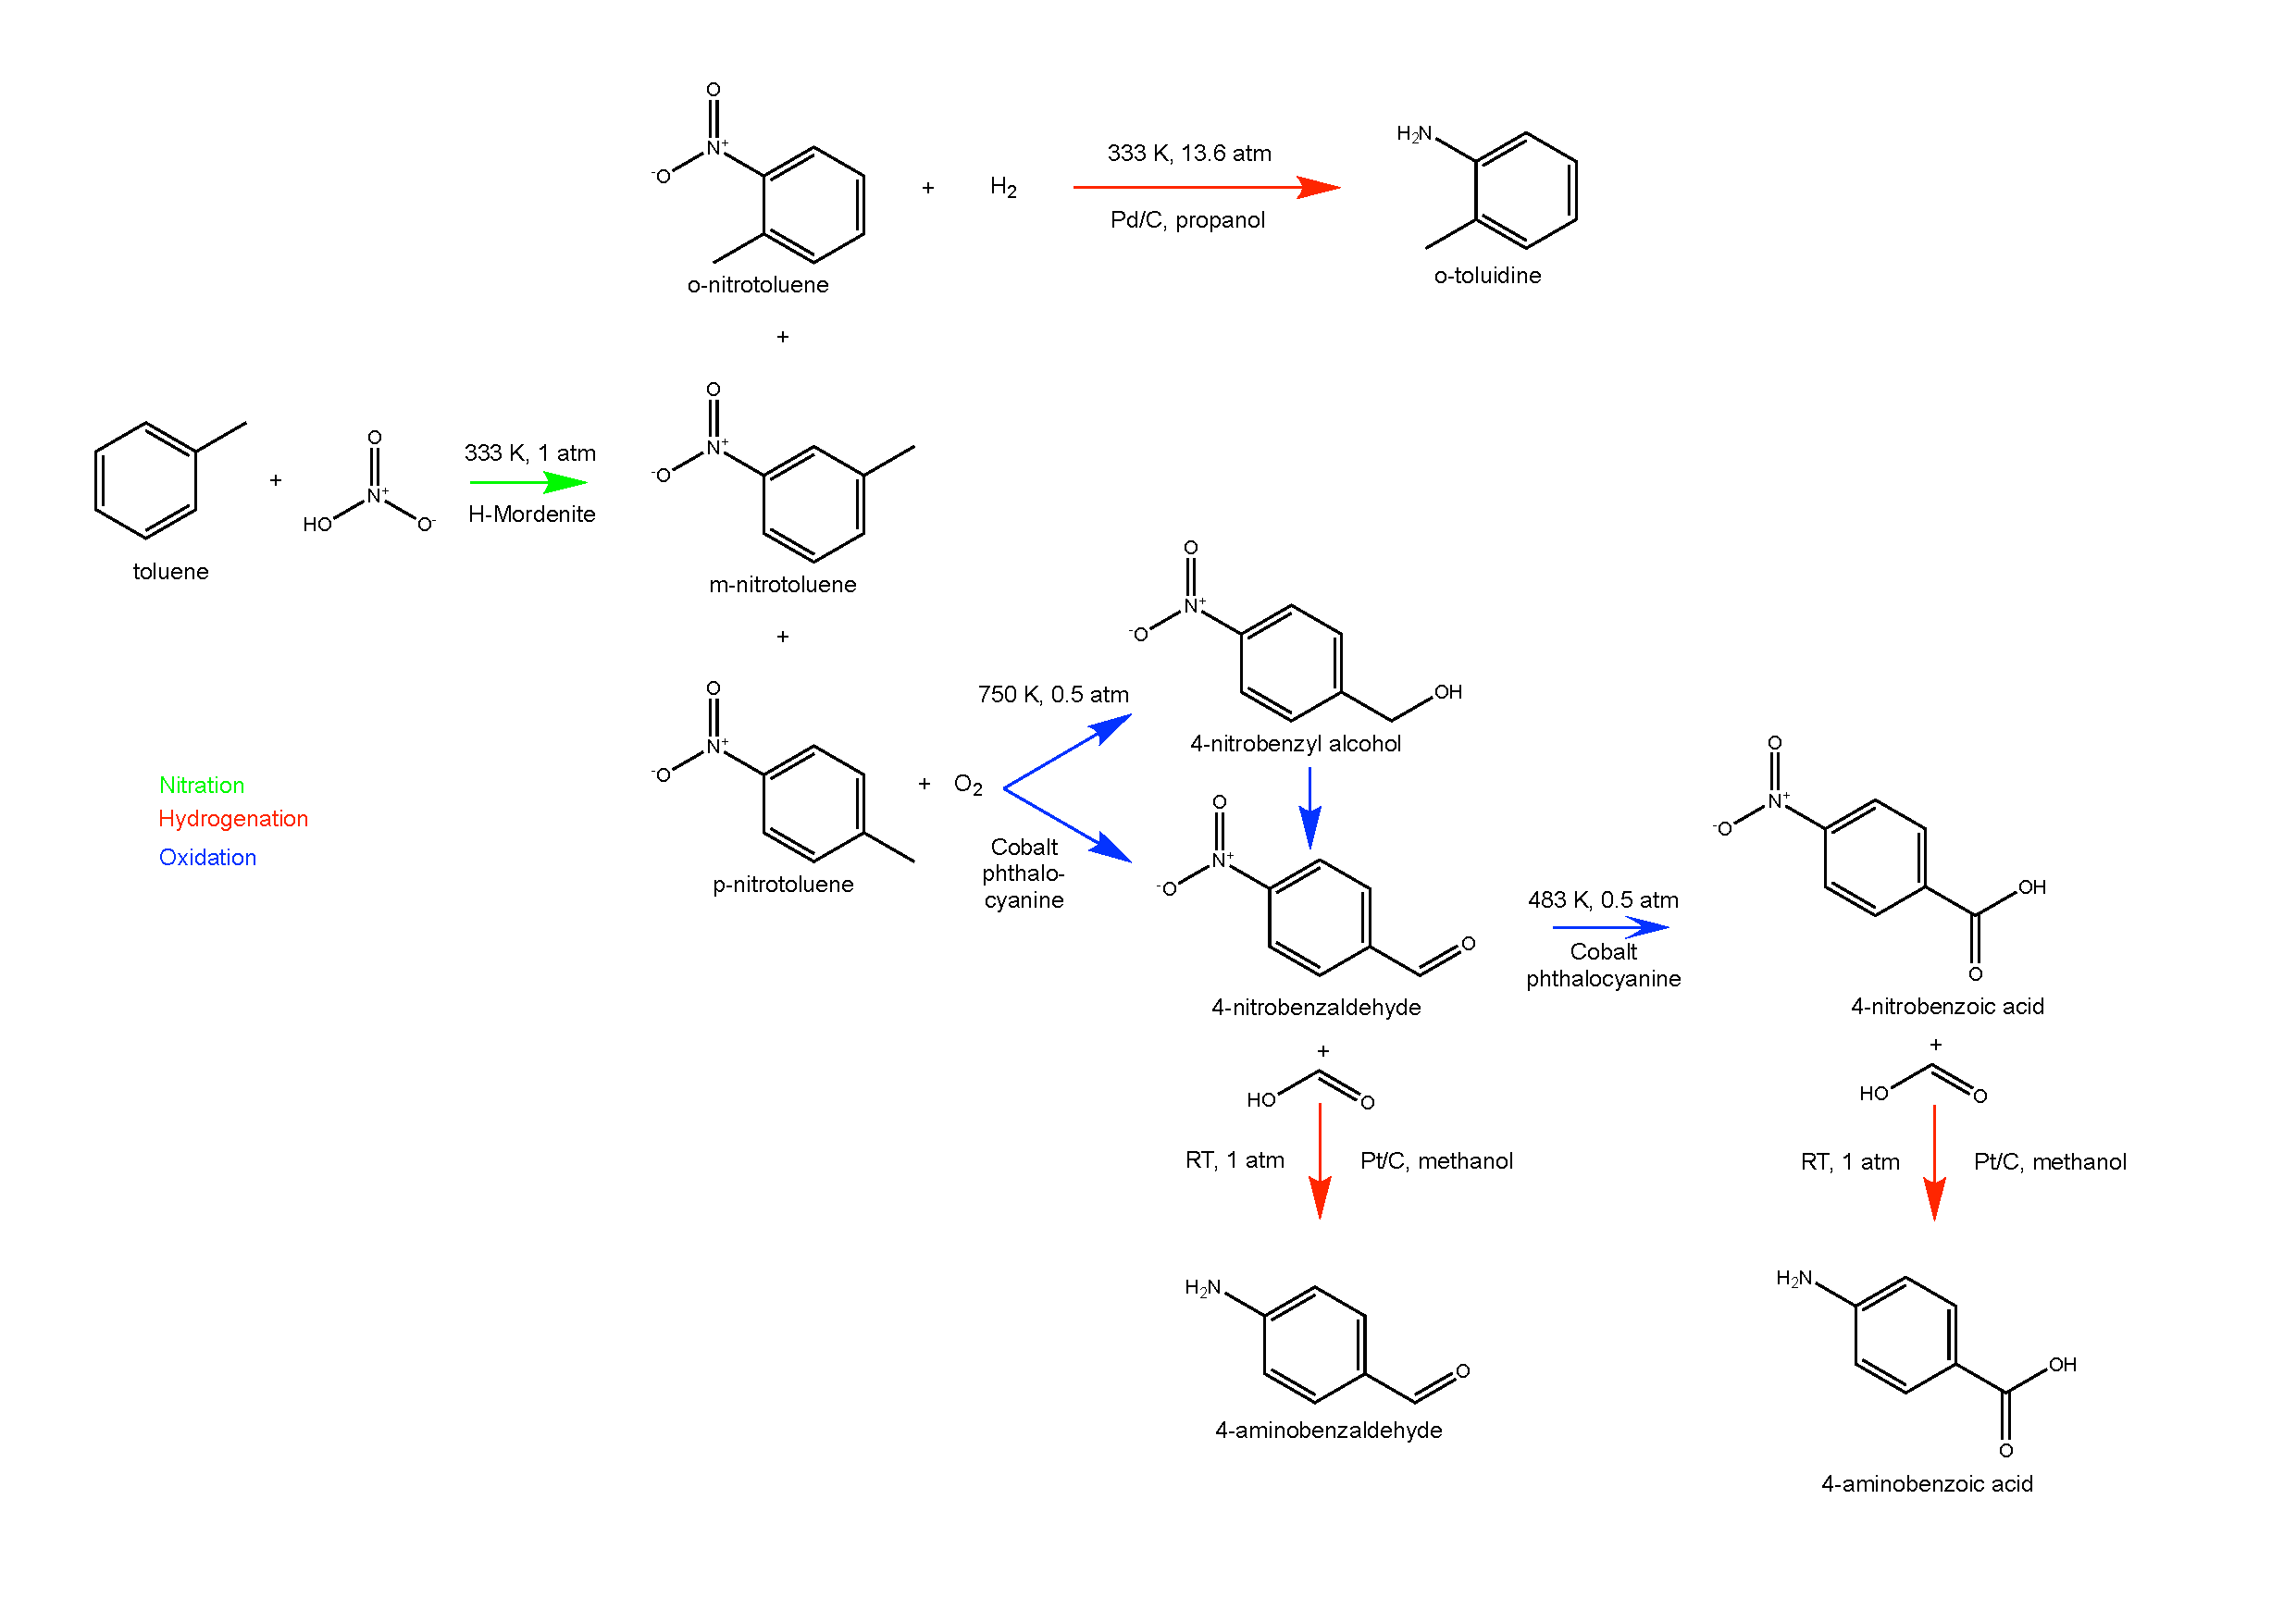
\includepdf[pages=-,landscape]{figures/routes-chosen.pdf}

\afterpage{\clearpage
\begin{landscape}
\begin{figure}
    \centering
    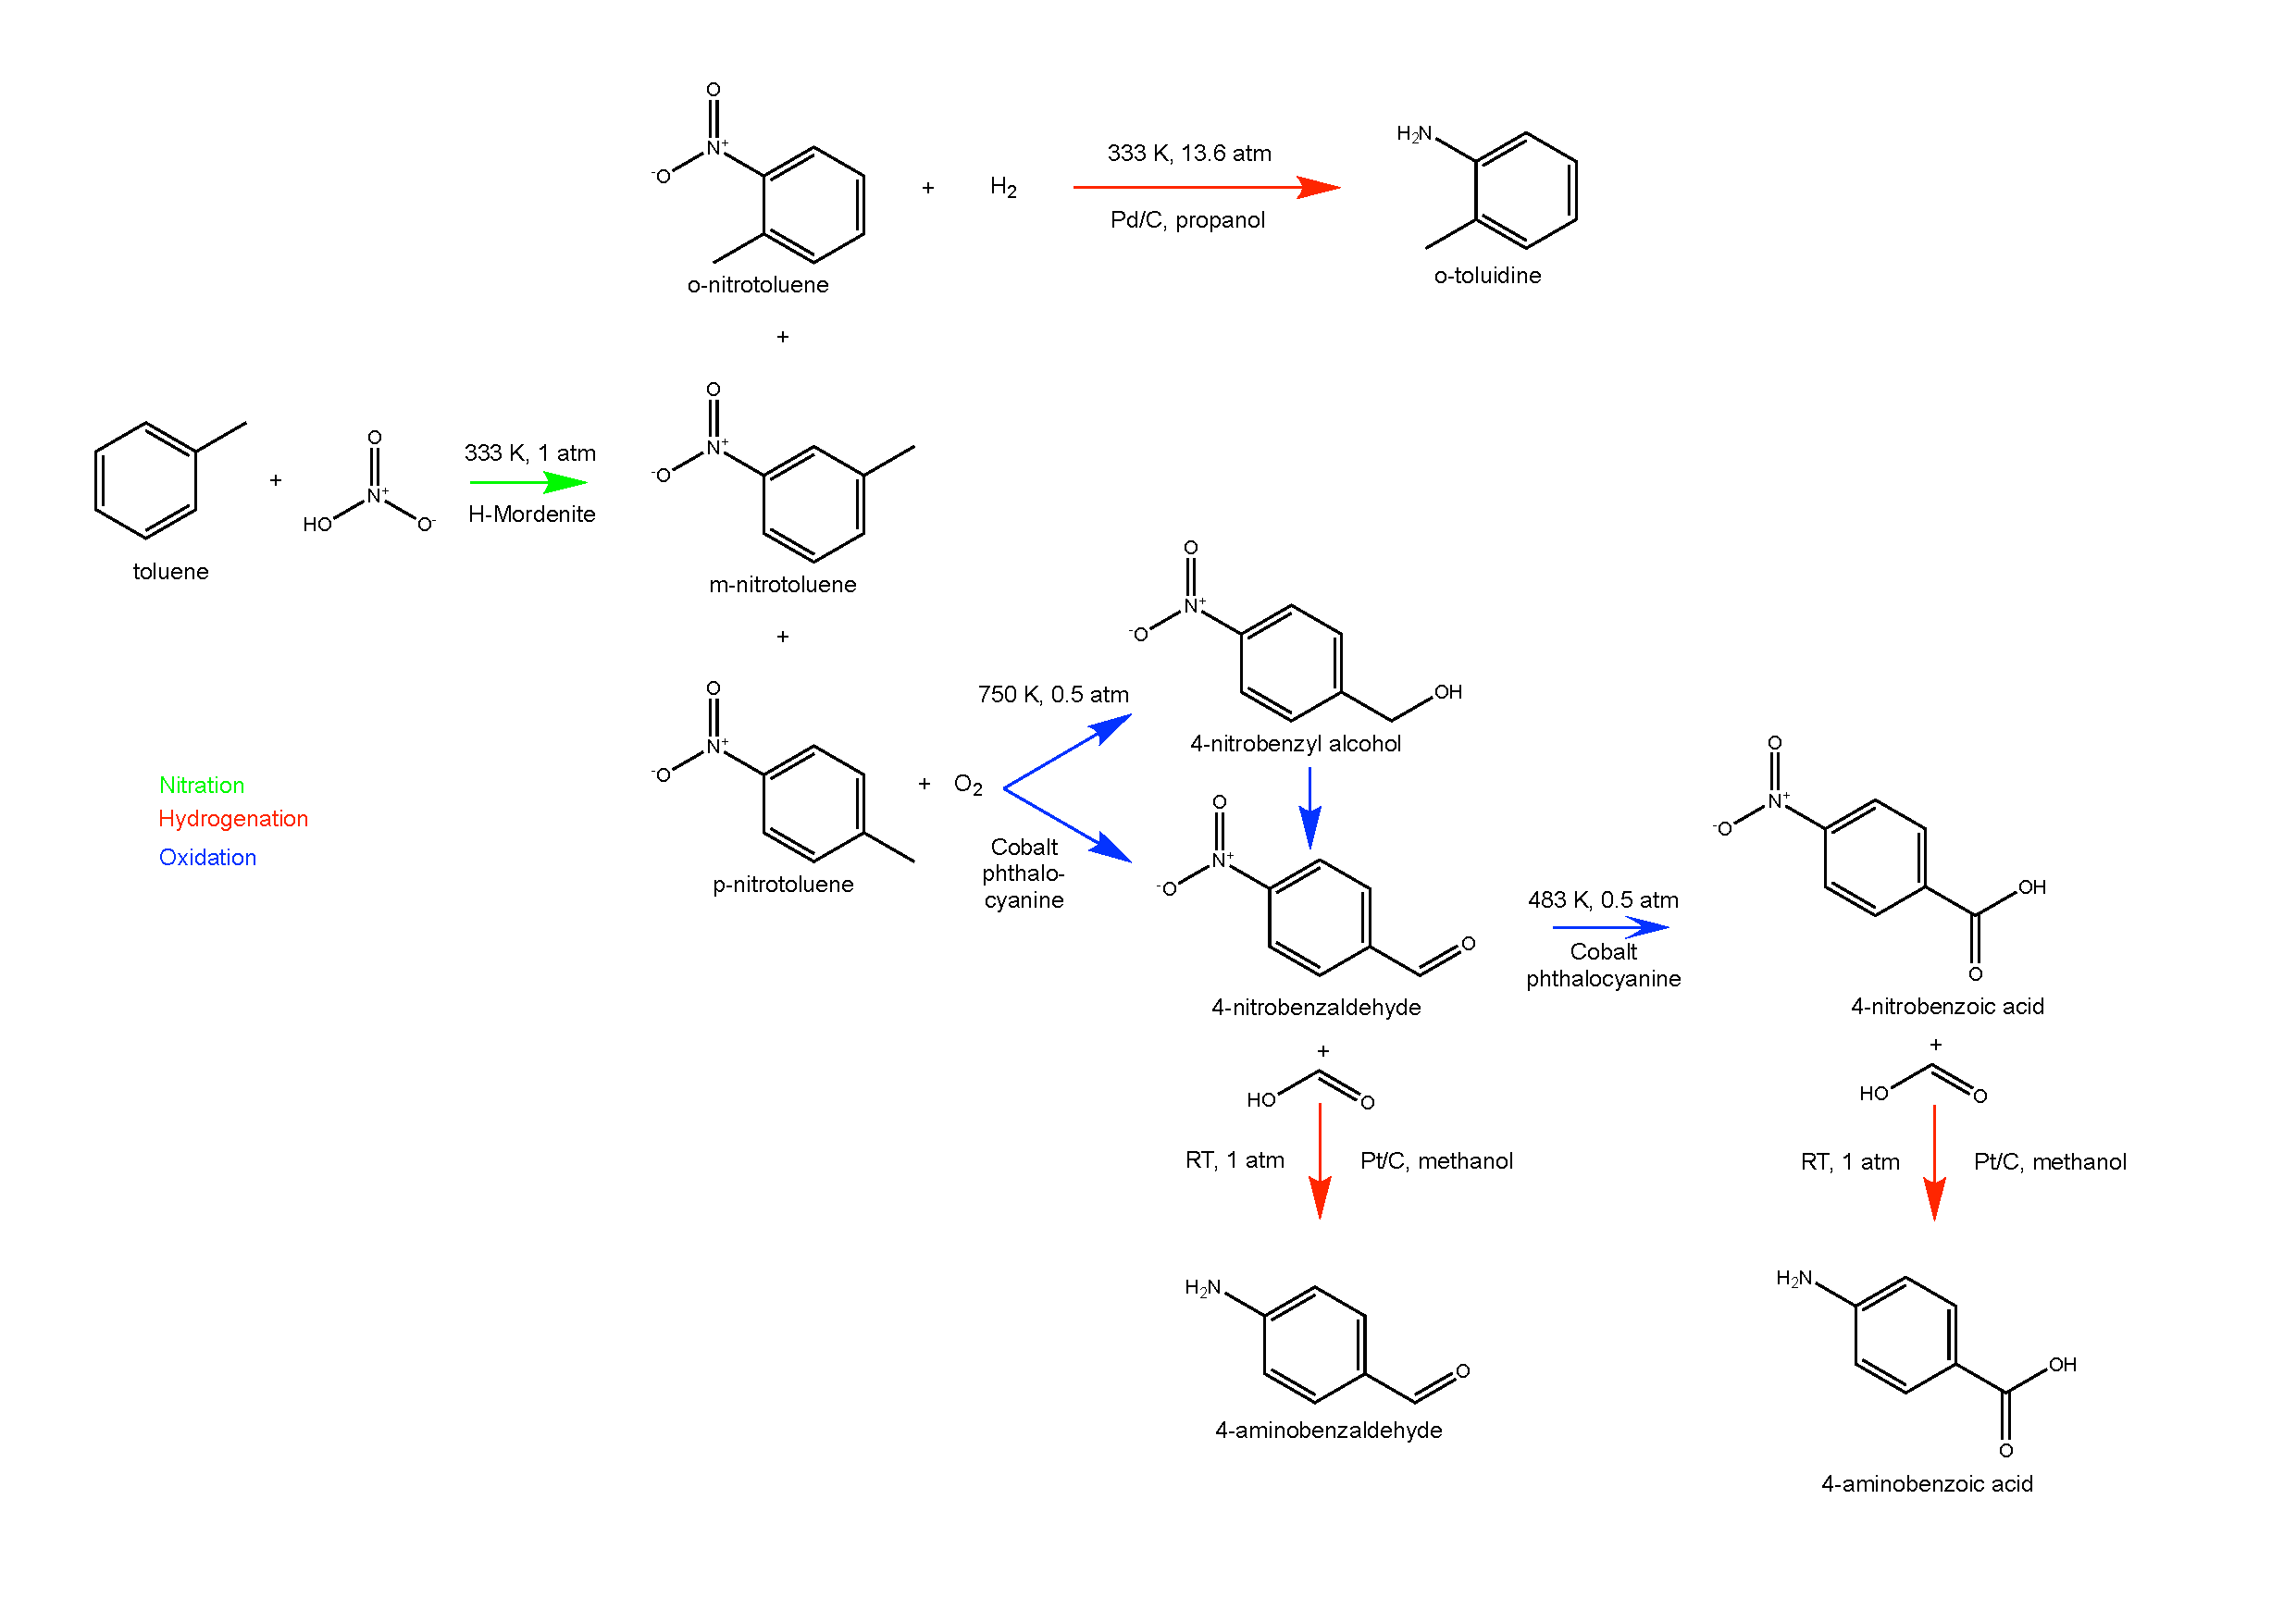
\includegraphics[width=0.8\linewidth]{figures/routes-chosen.pdf}
    \caption{Selected synthesis routes}
    \label{fig:routes-chosen}
\end{figure}
\end{landscape}
}

\end{document}
